\chapter{ PARTICLE TRANSPORT AND LAGRANGIAN DRIFTS}
\label{ch:part:transp}

\section{ Drogue Displacements}
\label{sec:drog:displ}
 During a hydrodynamic simulation, \telemac{2d} offers the possibility of monitoring the tracks followed by certain particles (drogues) introduced into the fluid from outflow points. The result is produced in the form of a Tecplot format file containing the various positions of the drogues in time, see paragraph \ref{subs:drog:output:file} for more details.

 Note that using this function provides more accurate results than using the particle tracking features of the post-processing tools. Contrary to \telemac{2d} for which monitoring floats is determined at each time step, the post-processing tools are based on the results file that is usually sampled much coarser. Since release 7.0 the management of drogues is modified to be coherent with other particle transport features of \telemac{2d} (oil spill and algae). Hereafter, we give the implementation details.

\subsection{ Input Files}
\label{subs:drog:inp:fil}
 In addition to the mandatory files for a classical \telemac{2d} model (steering, geometry boundary conditions), it is necessary to add a fortran file to run a particle transport case.

\subsection{ Steering file}
\label{subs:drog:steer:file}
 The steering file has to include the following key-words to account for drogue transport (for oil spill and algae, as well):

\begin{enumerate}
\item  The number of particles released: \textit{NUMBER OF DROGUES}, this is the maximum number used to dimension various arrays.

\item  The frequency of the drogues printout period: \textit{PRINTOUT PERIOD FOR DROGUES} \textit{;}

\item  The name of the output file (tecplot file) containing the drogue displacement: \textit{DROGUES FILE} (see section \ref{subs:drog:output:file});

\item  \telemac{2d} offers the possibility to introduce a stochastic diffusion coefficient. When setting the key-word \textit{STOCHASTIC DIFFUSION MODEL} =1 (default = 0), a stochastic model will generate stochastically a diffusion coefficient which is computed using the turbulent viscosity. If no turbulence is activated, this stochastic diffusion is not considered during the particle transport.
\end{enumerate}

\subsection{ Fortran file}
\label{subs:drog:fortr:file}
 Once the number of released drogues has been defined in the steering file, subroutine FLOT is used to define their positions and time of release. This is done by using the variable LT, which is the iteration step. This variable is used to release particles at a specific time. The subroutine ADD\_PARTICLE is then used to set the initial values of variables XFLOT, YFLOT and TAGFLOT, which are the two-dimensional position components and an identifier of the particle. An example of these changes can be found in subroutine FLOT (./sources/telemac2d). See also section \ref{sec:oil:spill:modell}.

 \textbf{Modifications to subroutine }FLOT\textbf{:}

\begin{enumerate}
\item \textbf{ }Use LT to define when to release particles

\item  Call ADD\_PARTICLE to define XFLOT, YFLOT and TAGFLOT
\end{enumerate}


\subsection{ Output file}
\label{subs:drog:output:file}
 Besides the classic result file, \telemac{2d} produces a specific output file for drogues. It is given by the key-word \textit{DROGUES FILE. }

 This file is a formatted file created by \telemac{2d} during the computation. It stores drogue positions in TECPLOT format. To visualize the drogue positions with Tecplot software, the user must:

\begin{enumerate}
\item  Use the File$>$Load Data File(s) command to load the 2D RESULT FILE

\item  Use the File$>$Load Data File(s) command to load the Tecplot drogue file
\end{enumerate}

\begin{WarningBlock}{Warning:}
 In order to add the Tecplot DROGUE FILE to Telemac result data that was already loaded, select ``Add to current data'' set in the \textbf{Load Data File Warning dialogue} (cf. Figure \ref{fig:load:df}). The Load Data File Warning dialogue will appear after you have selected the file and zones and/or variables to load.
\end{WarningBlock}
\begin{figure}
\centering
 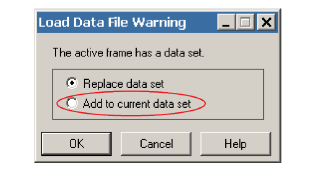
\includegraphics[width=2.77in, height=1.70in, keepaspectratio=false]{./graphics/warning1.png}
 \caption{Warning dialogue box}%
 \label{fig:load:df}
\end{figure}

 \textbf{Change the drogue output format:}

 It is possible to develop a new drogue output format. This must be done in the subroutine DERIVE. A Fortran file including the subroutine DERIVE with the new format definition for the DROGUE FILE needs to be added with the input files.


\section{ Algae bloom modelling}
\label{sec:algae:bloom}
 Since release 6.3, \telemac{2d} offers the possibility to simulate algae bloom transport. Theoretical aspects about algae physics and modelization can be found in Joly \cite{Joly2011}.


\subsection{Input files}

 Input files for algae bloom modelling are the same than for drogues.


\subsection{ Steering file}

 The steering file has to include the following key-words to account for an algae bloom propagation model:

\begin{itemize}
\item  The number of particle released: \textit{NUMBER OF DROGUES};

\item  The frequency of the algae printout period: \textit{PRINTOUT PERIOD FOR DROGUES};

\item  The name of the output file (tecplot file) containing the drogue displacement: \textit{DROGUES FILE} (see section \ref{subs:drog:output:file});

\item  The option setting the particles as algae: \textit{ALGAE TRANSPORT MODEL=YES} (default\textit{ = NO});

\item  The type of algae particles considered \textit{ALGAE TYPE} (default 1). The different choices are:

\begin{enumerate}
\item Sphere,

\item Iridaea Flaccida,

\item Pelvetiopsis Limitata,

\item Gigartina Leptorhynchos
\end{enumerate}

\item  The physical properties of the algae (diameter, density and thickness):

\begin{itemize}
\item  \textit{DIAMETER OF ALGAE} (default = 0.1);

\item  \textit{DENSITY OF ALGAE} (default = 1050);

\item  \textit{THICKNESS OF ALGAE} (default = 0.01).
\end{itemize}
\end{itemize}

\begin{WarningBlock}{Warning:}

\begin{itemize}
\item  Even though some of the previous keywords make references to drogues, they are also used for algae blooms.

\item  To use the algae particle transport module it is necessary to use the k-$\epsilon$ turbulence model, i.e. the option \textit{TURBULENCE MODEL = 3} needs to be set in the steering file.
\end{itemize}
\end{WarningBlock}

\subsection{Fortran file}

 Once algae transport has been defined in the steering file, the subroutine FLOT is used to define the position and time of release. This is done by defining the variable ALGAE\_START and using the variable LT to release particles. In addition the subroutine ADD\_PARTICLE is used to set the initial values of variables XFLOT, YFLOT and TAGFLOT, which are the two-dimensional position components and an identifier of the particle. An example how to use FLOT to release algae particles is put in comments within the subroutine FLOT.

 \textbf{Modifications to subroutine for algae transport}

\begin{enumerate}
\item Add the command USE ALGAE\_TRANSP at the beginning of the routine

\item  Define ALGAE\_START, which will be used as the release time of the algae (so far a simple time release is allowed)

\item  Use LT to release particles

\item  Call ADD\_PARTICLE to define XFLOT, YFLOT and TAGFLOT
\end{enumerate}

\begin{WarningBlock}{Warning:}
\begin{itemize}
\item  ALGAE\_START needs to be greater or equal to 1

\item  So far, it is possible to achieve a unique release of algae. To do multiple releases (in different times), futher developments are necessary.
\end{itemize}
\end{WarningBlock}

\subsection{ Output files}

 Likewise for drogues, see \ref{subs:drog:output:file}.


\section{ Oil spill modelling}
\label{sec:oil:spill:modell}
 A new feature has been added to \telemac{2d} (and 3D) that allows the simulation of oil spill problems. These developments are based on the work of Goeury \cite{goeury2012}.


\subsection{ Input files}

 In addition to the minimum set of input files necessary to run a \telemac{2d} case, an oil spill computation needs also an oil spill steering file. Furthermore, to run oil spill model a FORTRAN file including the routine OIL\_FLOT needs to be added.


\subsection{ Steering file}

 The following essential information should be specified in the \telemac{} steering file to run an oil spill propagation model:

\begin{itemize}
\item  The use of the oil spill model must be declared: \textit{OIL SPILL MODEL = YES} (default\textit{ = NO});

\item  The name of the oil spill steering file which contains the oil characteristics: \textit{OIL SPILL STEERING FILE};

\item  The number of oil particles to be released during the oil spill episode: \textit{NUMBER OF DROGUES};

\item  The frequency of the drogues printout period: \textit{PRINTOUT PERIOD FOR DROGUES};

\item  The name of the Tecplot file containing the oil displacement: \textit{DROGUES FILE}.
\end{itemize}

\begin{WarningBlock}{Warning:}
\begin{itemize}
\item  Even though some of the previous keywords make references to drogues, they are also used for algae blooms and oil spills.

 With the oil spill module, it is possible to take into account the transport of soluble oil components in water (whose presence has no effect on the hydrodynamics). These may or may not be diffused within the flow but their characteristics have to be defined in the \textit{OILSPILL STEERING FILE.} If these components are allowed to diffuse in the flow they are then treated with the tracer transport computations of \telemac{2d}. This implies that the logical keyword \textit{TRACER} is set to \textit{YES} and the \textit{NUMBER OF TRACER} must be set to the number of the oil soluble components. In addition, \textit{TRACER} keywords, enunciated in the Chapter \ref{ch:tra:trans} can be specified.

\item If the number of oil components dissolved in water is greater than 1, the result file can contain the sum of dissolved oil concentrations. The user must only add the variable for graphic printout N:

\textit{VARIABLES FOR GRAPHIC PRINTOUTS: '....,N'}

With the variable for graphic printout \textbf{\textit{N}}, be careful not to have private tables or change the table PRIVE1 in the subroutine PRERES\_TELEMAC2D.f by the table PRIVEX (where X is the number chosen by the user).
\end{itemize}
\end{WarningBlock}

\subsection{ Oil spill steering file}

 As seen previously, the \textit{OIL SPILL STEERING FILE }name is given by the user in the \telemac steering file. This file contains all information on oil calculation based on the composition considered by the user:

\begin{enumerate}
\item  The number of non-soluble components in oil,

\item  The parameters of these components such as the mass fraction (\%) and boiling point of each component (K),

\item  The number of soluble components in oil,

\item  The parameters of these components such as the mass fraction (\%), boiling point of each component (K), solubility (K${}_{g}$.m${}^{-3}$) and the mass transfer coefficient of the dissolution and volatilization phenomena (m.s${}^{-1}$),

\item  The oil density,

\item  The oil viscosity (m${}^{2}$.s${}^{-1}$),

\item  The volume of the spilled oil (m${}^{3}$),

\item  The water surface temperature (K),

\item  The spreading model chosen by the user:

\begin{enumerate}
\item  Fay's model,

\item  Migr'Hycar model,

\item  Constant area model.
\end{enumerate}
\end{enumerate}

\begin{WarningBlock}{Warning:}
\begin{itemize}
\item The parameters of soluble (or non-soluble) components need to be informed only if the number of these components is not null,

\item  If the sum of all mass fraction components is not equal to 1, the run is interrupted and an error message is displayed:

 ''WARNING::THE SUM OF EACH COMPONENT MASS FRACTION IS NOT EQUAL TO 1.''

 ``PLEASE, MODIFY THE INPUT STEERING FILE''
\end{itemize}
\end{WarningBlock}

An example of the oil spill steering file is given.
\begin{lstlisting}[language=bash]
NUMBER OF UNSOLUBLE COMPONENTS IN OIL
6
UNSOLUBLE COMPONENTS PARAMETERS (FRAC MASS, TEB)
5.1D-02    ,402.32D0
9.2D-02    ,428.37D0
3.16D-01   ,458.37D0
3.5156D-01    ,503.37D0
8.5D-02       ,543.37D0
9.4D-02       ,628.37D0
NUMBER OF SOLUBLE COMPONENTS IN OIL
4
SOLUBLE COMPONENTS PARAMETERS(FRAC MASS, TEB, SOL, KDISS, KVOL)
1.D-02   ,497.05D0,  0.018D0   , 1.25D-05 ,5.0D-05
3.2D-02  ,551.52D0,  0.00176D0 , 5.63D-06 ,1.51D-05
1.D-04   ,674.68D0,  2.0D-04   , 2.D-06   ,4.085D-07
2.D-05   ,728.15D0,  1.33D-06  , 1.33D-06 ,1.20D-07
OIL DENSITY
830.D0
OIL VISCOSITY
4.2D-06
OIL SPILL VOLUME
2.02D-05
WATER TEMPERATURE
292.05D0
SPREADING MODEL(1=FAY'S MODEL,2=MIGR'HYCAR MODEL,3=CONSTANT AREA)
2
\end{lstlisting}
If in the oil spill steering file, the SPREADING MODEL is set to 3, two lines must be added to the previous example:
\begin{lstlisting}[language=bash]
CONSTANT AREA VALUE CHOSEN BY THE USER FOR EACH OIL PARTICLE
1
/example if the user wants area particle equal to 1 m2
\end{lstlisting}
\subsection{ The oil\_flot subroutine}

 After inserting the OIL\_FLOT subroutine in the FORTRAN file, the user must modify it in order to indicate the release time step, together with the coordinates of the release point. If the release point coordinates are outside the domain, the run is interrupted and an error message is displayed. In addition, if a particle leaves the domain during the simulation, it is of course no longer monitored but its previous track remains in the results file for consultation.

 An example of modifications in the OIL\_FLOT subroutine is given.

 The release time step in the first condition statement and the coordinates of the release point must be changed:
\begin{lstlisting}[language=TelFortran]
...
IF(LT.EQ.10000)THEN
  NUM_GLO=0
  NUM_MAX=0
  NUM_LOC=0
  COORD_X=0.D0
  COORD_Y=0.D0
  NUM_MAX=INT(SQRT(REAL(NFLOT_MAX)))
  DO K=1,NUM_MAX
    DO J=1,NUM_MAX
      COORD_X=336000.D0+REAL(J)
      COORD_Y=371000.D0+REAL(K)
      NUM_GLO=NUM_GLO+1
      NFLOT_OIL=0
      CALL ADD_PARTICLE(COORD_X,COORD_Y,0.D0,NUM_GLO,NFLOT_OIL,
&                       1,XFLOT,YFLOT,YFLOT,TAGFLO,
&                       SHPFLO,SHPFLO,ELTFLO,ELTFLO,MESH,1,
&                       0.D0,0.D0,0.D0,0.D0,0,0)
...
    END DO
  ENDDO
END IF
\end{lstlisting}

\subsection{ Output files}

 There are no additional output files provided than for drogue transport.

\begin{WarningBlock}{Warning:}
 If the user wants to develop a new drogue output format for oil spill, he must edit subroutine OIL\_DERIVE.f and not the subroutine DERIVE.f used for the drogue and algae transport.
\end{WarningBlock}

\section{ Lagrangian drifts}
\label{sec:lagr:drifts}

\subsection{ Input files}

 Computing Lagrangian drifts involves computing the displacement of all mesh points between two given instants. Typically, these two instants may be two consecutive high tides.

 To run such a computation, it is necessary to program the steering file and FORTRAN file.

 In the steering file, the user must firstly provide the number of drifts required using the keyword \textit{NUMBER OF LAGRANGIAN DRIFTS} (default value 0). This value corresponds to the number of pairs (starting and ending times) for which the Lagrangian drifts are computed. Secondly, the user must include the letters A and G in the list assigned to the keyword \textit{VARIABLES FOR GRAPHIC PRINTOUTS}. These two letters correspond to the drift displacements along X and Y.

 As far as the FORTRAN file is concerned, the user must insert the LAGRAN subroutine, in which it is necessary to define the instants at which each computation is to start and end, in the form of time step numbers.

 The drift computation results are stored directly in the \telemac{2d} results file in the form of two scalar variables entitled DRIFT\_ALONG\_X and DRIFT\_ALONG\_Y. Given the possible discretization that may occur in printing out graphical results, the rule for introduction in the results file is the following:

\begin{itemize}
\item  If none of the drift computations is completed at the time step considered, the two variables are set to zero.

\item  Otherwise, the two variables contain the results of the most recently completed drift computation.
\end{itemize}

 This means on one hand that two drifts may not be completed at the same time step, and on the other hand that between two ends of drift computations, a record must be made in the results file (otherwise the result of the first computation is lost).

 Lastly, if a drift leaves the domain, the corresponding computation is interrupted and the result reset at zero for this node.


\subsection{ Output files}

 The result is produced in the form of a Serafin format file containing the various positions of the lagrangian drifts in the form of a degenerated mesh.



  The following example (steering file and FORTRAN file) carries out two drift computations. The first begins at time step 10 and finishes at time step 50. The second begins at time step 15 and finishes at time step 40.

  In the steering file:
\begin{lstlisting}[language=bash]
NUMBER OF LAGRANGIAN DRIFTS     = 2
VARIABLES FOR GRAPHIC PRINTOUTS = 'U,V,H,A,G'
GRAPHIC PRINTOUT PERIOD         = 1
\end{lstlisting}
  In the LAGRAN subroutine of the FORTRAN file:
\begin{lstlisting}[language=TelFortran]
DEBLAG(1) = 10
FINLAG(1) = 50
DEBLAG(2) = 15
FINLAG(2) = 40
\end{lstlisting}
 In this example, the variables DRIFT\_ALONG\_X and DRIFT\_ALONG\_Y of the results file will contain the following values:

\begin{itemize}
\item  From time steps 1 to 39: 0 values (no finished drift computation).

\item  From time steps 40 to 49: results of the second drift computation.

\item  Time step 50: results of the first drift computation.
\end{itemize}

 NOTE: Lagrangian drifts are not yet implemented for parallelism.

